\documentclass[a4paper, 12pt]{article}
\usepackage[english]{babel}
\usepackage[margin=1in]{geometry}
\usepackage{graphicx}
\usepackage{setspace}
\usepackage{multicol}
\usepackage{float}
\usepackage{subfig}
\usepackage{wrapfig}
\usepackage{hyperref}
\usepackage{booktabs}
\usepackage{gensymb}
\usepackage{csquotes}

\doublespacing

\graphicspath{{img}}

\setcounter{section}{-1}

\title{\Large EEE102 - 03 \qquad Lab Report 01\\ \small \hrulefill}
\date{}
\author{Selim Mert TOKER 22302352}

\begin{document}

\maketitle

\section{Introduction}

Oscilloscopes are electronic measurement devices that measure and plot voltage over time very quickly.
A typical oscilloscope can take samples (measures voltage) millions of times a second to accurately show high-frequency or short-duration signals an electronic engineer may want to see.
This is why the oscilloscope is such an important device for learning and practicing electronics.
This lab session aims to explore how an oscilloscope works and what are its limitations, in 6 experiments.

\section{Tuning an Oscilloscope Probe}

\begin{wrapfigure}{r}{0.4\textwidth}
	\vspace{-1cm}
	\centering
	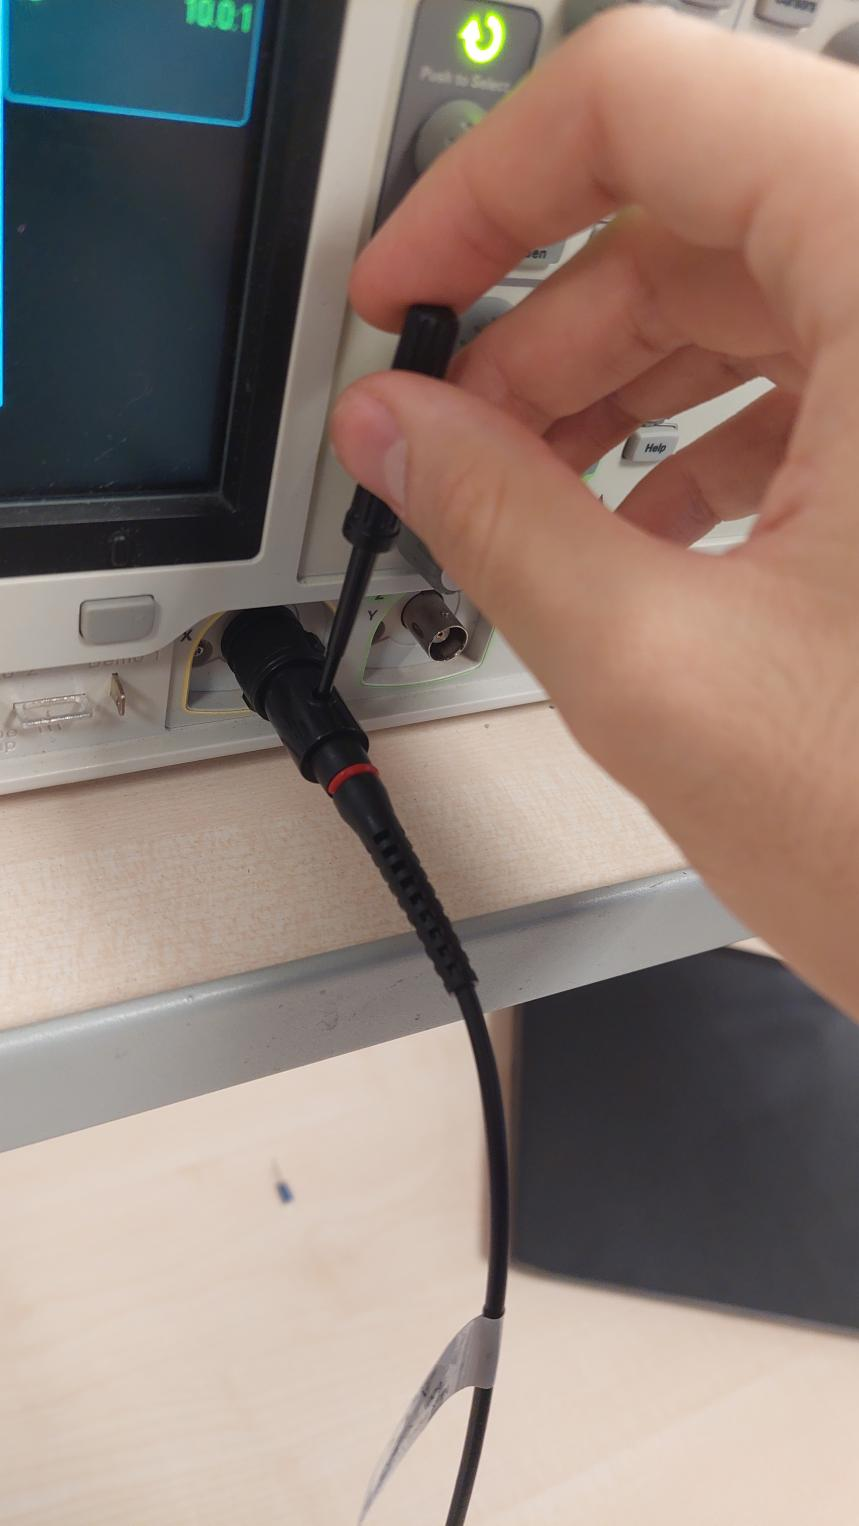
\includegraphics[width=0.3\textwidth]{1.0.jpg}
	\caption{Tuning the Probe}
	\label{fig:probe-comp}
\end{wrapfigure}

The probes, measurement wires of the oscilloscope, have some parasitic capacitance and inductance, which may change the original signal being measured.
That is why the probes have to be compensated (tuned) to mitigate the related errors.
On the probes, there usually is a screw, which lets us tune the amount of this compensation.
In order to tune the probe, there usually is a 1kHz square wave signal provided by the oscilloscope which the probe is attached as shown in figure \ref{fig:probe-comp}.

\newpage

\mbox{Figure \ref{fig:comp-signal} shows the difference between compensated and uncompensated probes.}
\mbox{Although they are probing the same signal, the corners of the square wave are bent}, which is fixed after tuning the probes.

\begin{figure}[!h]
	\centering
	\subfloat[Uncompensated]{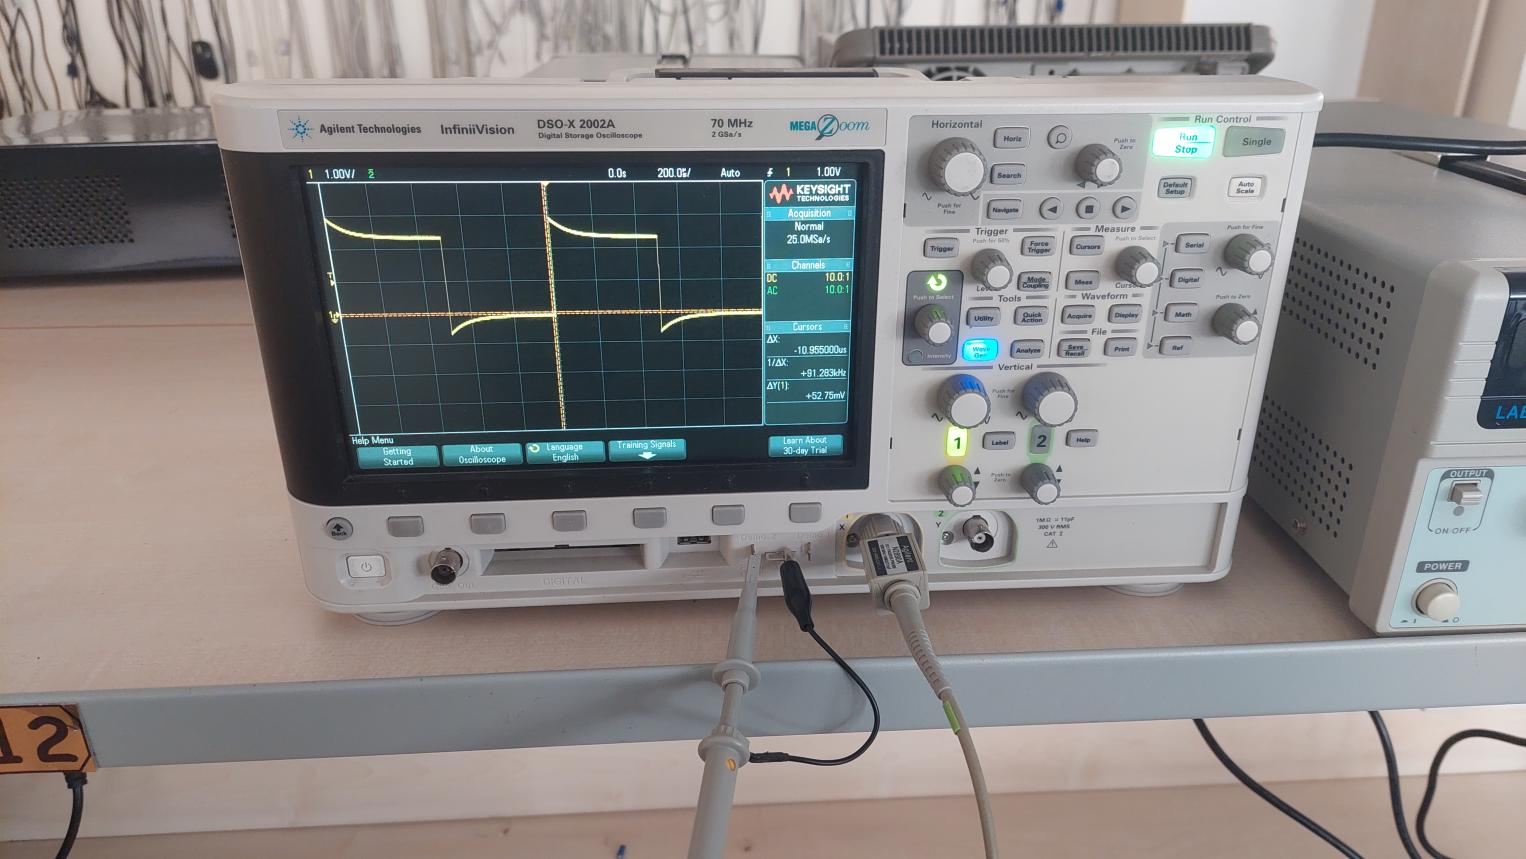
\includegraphics[width=0.48\textwidth]{1.1.jpg}}
	\hfill
	\subfloat[Compensated]  {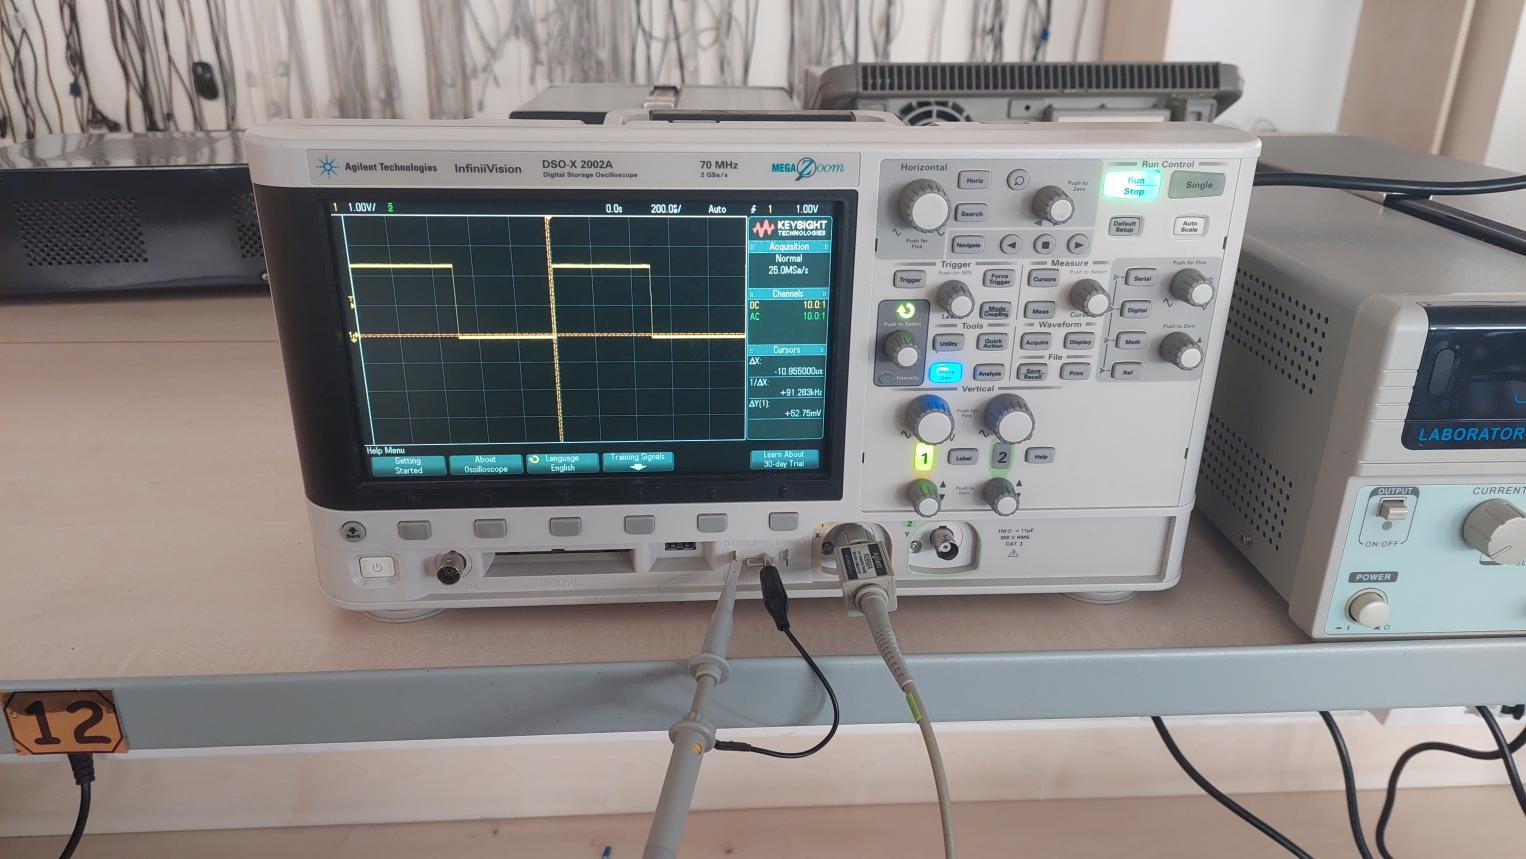
\includegraphics[width=0.48\textwidth]{1.2.jpg}}
	\caption{}
	\label{fig:comp-signal}
\end{figure}

\vspace{-1.5cm}
\section{Edge Triggering}

The oscilloscope, always listening the signal input, only draws the signal to the screen when a special event (trigger) occurs in the signal, which is either the voltage increasing above or dropping below a certain treshold value.
The exact moment the trigger occurs is aligned to be in a pre-determined point on the screen by the oscilloscope, so when edge triggering is set to rising/falling edge triggering, the oscilloscope looks for a voltage rise/drop above/below a certain value.

For the experiment, the oscilloscope is hooked up to a signal generator, outputting a 1kHz 5Vpp sine wave.
Figure \ref{fig:rifa-edge} shows the effect of the triggering edge, as rising edge makes the increasing edge of the sine wave appear on the middle line and vice versa.

\begin{figure}[!h]
	\centering
	\subfloat[Rising Edge] {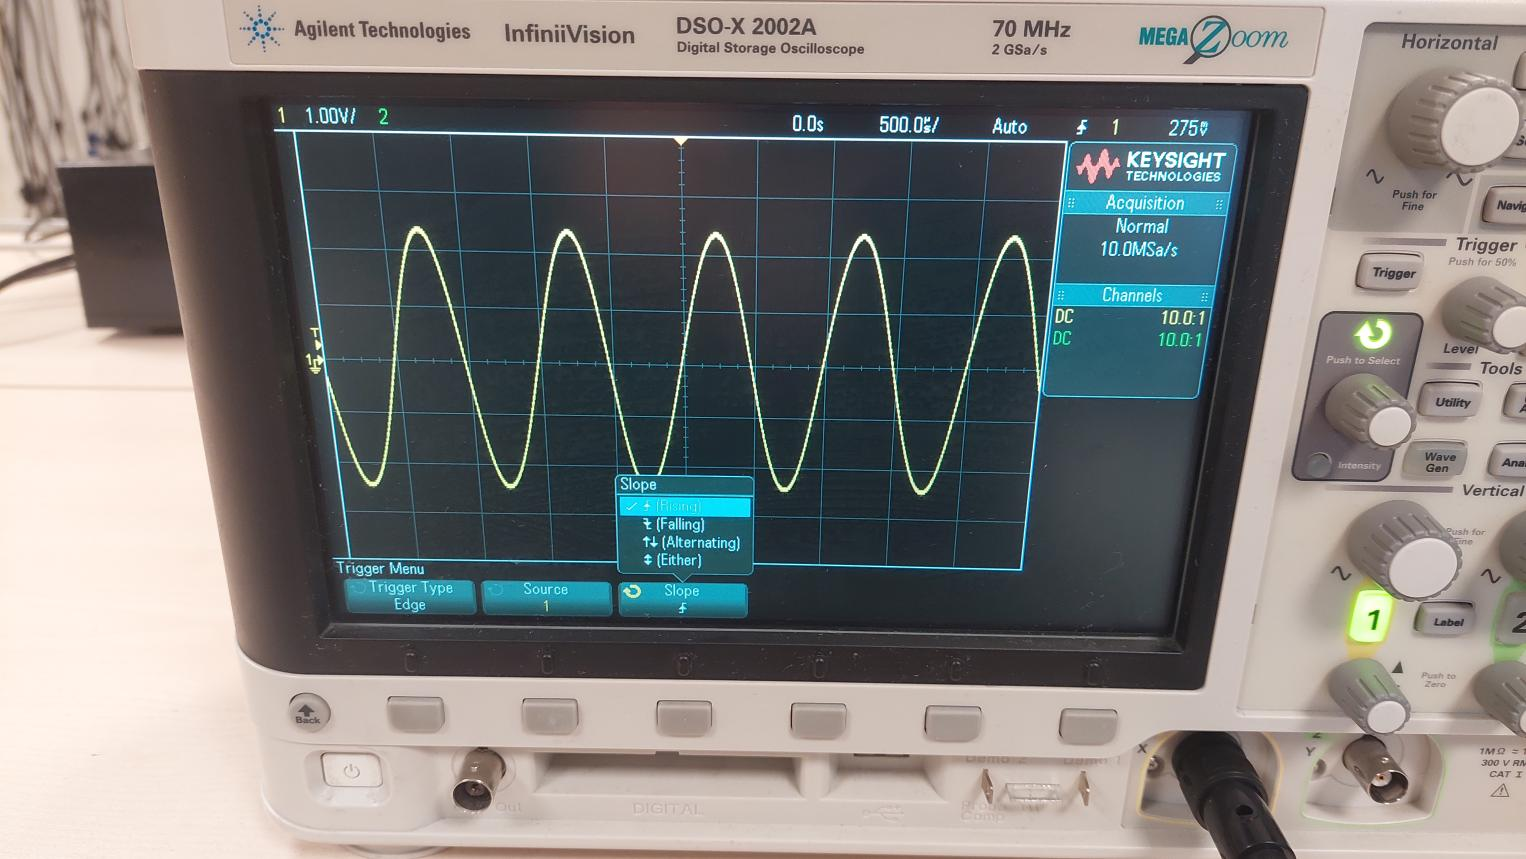
\includegraphics[width=0.48\textwidth]{2.1.jpg}}
	\hfill
	\subfloat[Falling Edge]{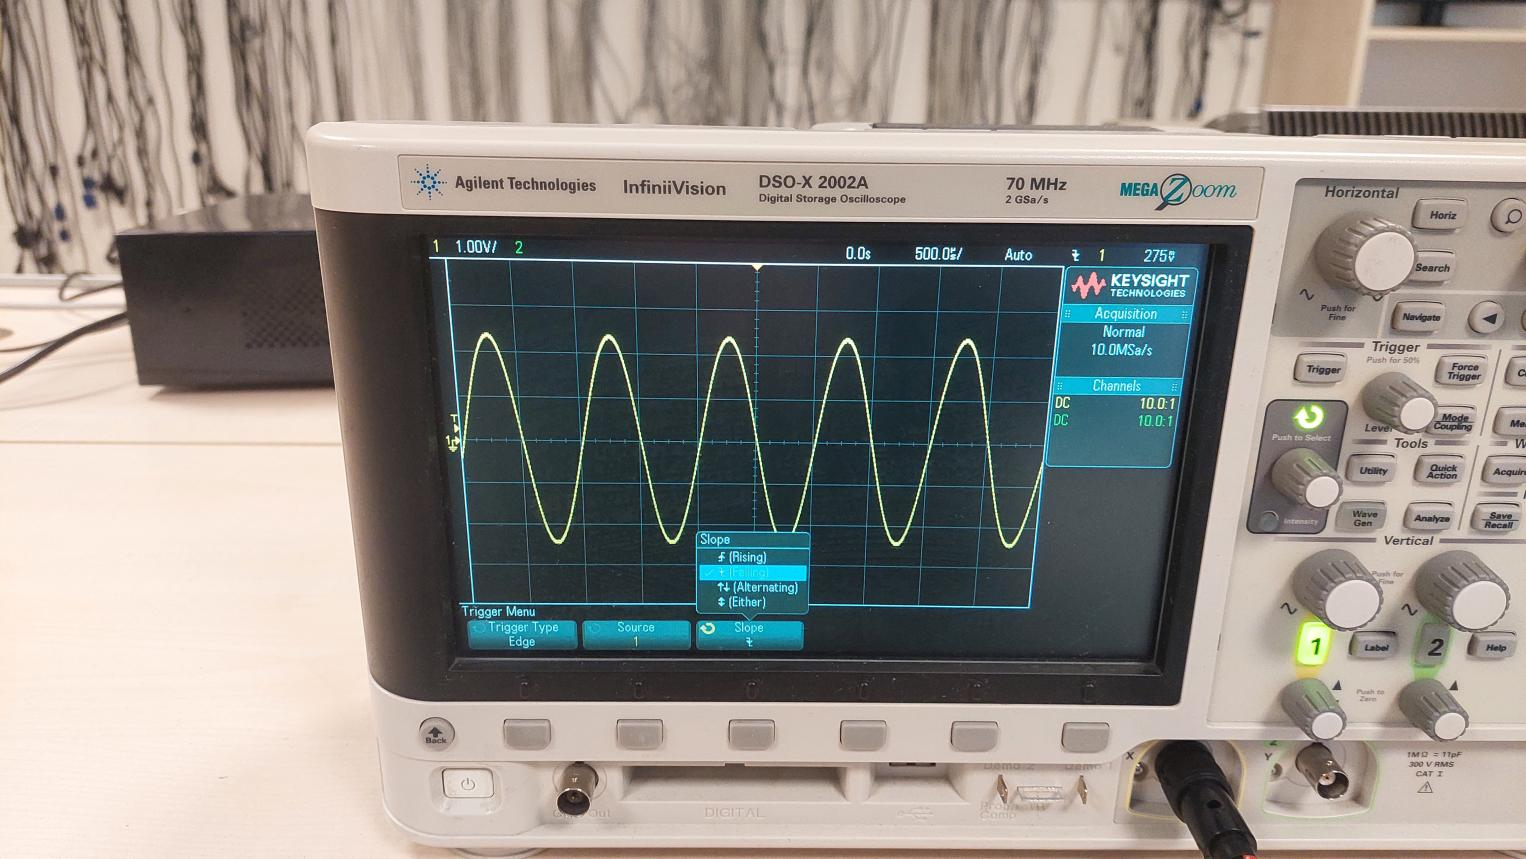
\includegraphics[width=0.48\textwidth]{2.2.jpg}}
	\caption{}
	\label{fig:rifa-edge}
\end{figure}

\section{Triggering Voltage}

As discussed in the previous experiment, the trigger voltage (indicated with "T" on the y-axis) is the voltage level which needs to be crossed to trigger the oscilloscope.
The oscilloscope aligns the signal plot on the screen so that the moment which the signal's voltage crosses the trigger voltage, is in the middle of the screen.

\begin{wrapfigure}{r}{0.5\textwidth}
	\centering
	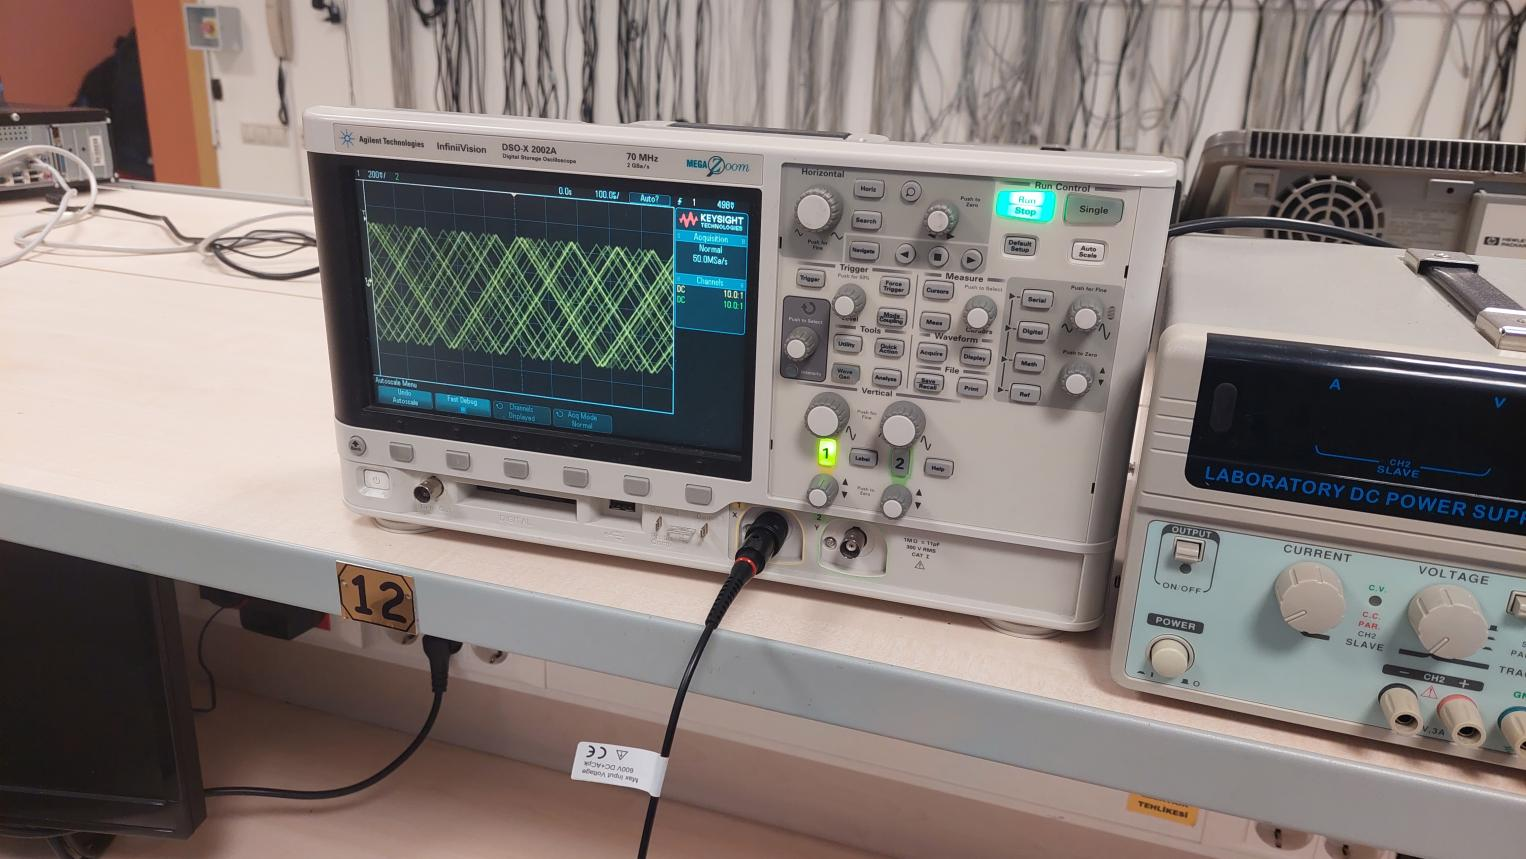
\includegraphics[width=0.4\textwidth]{3.3.jpg}
	\caption{Improper Trigger Voltage}
	\label{fig:bad-trig}
\end{wrapfigure}

The oscilloscope aligning the signal is extremely useful for being able to investigate the signal, and if it is not set properly, the oscilloscope can only show jittery lines as seen on figure \ref{fig:bad-trig}.
For the triangle wave (2kHz 1Vpp) used in this experiment, turning the trigger knob changes the phase of the signal or shifts the signal right and left, as seen in figure \ref{fig:trig-volt}.

\begin{figure}[!h]
	\centering
	\subfloat[Lower Trigger Voltage] {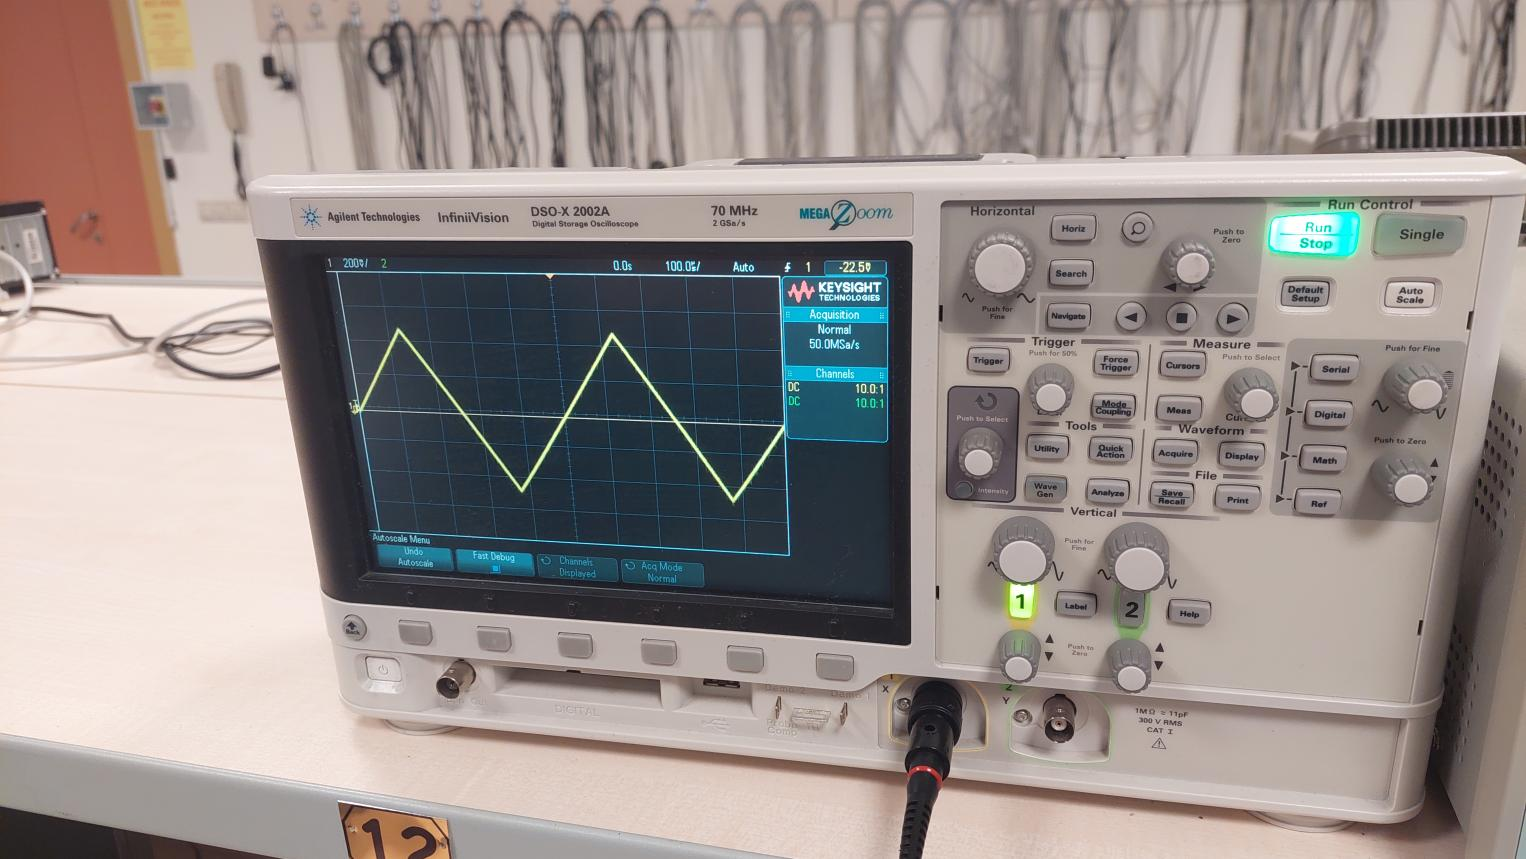
\includegraphics[width=0.48\textwidth]{3.1.jpg}}
	\hfill
	\subfloat[Higher Trigger Voltage]{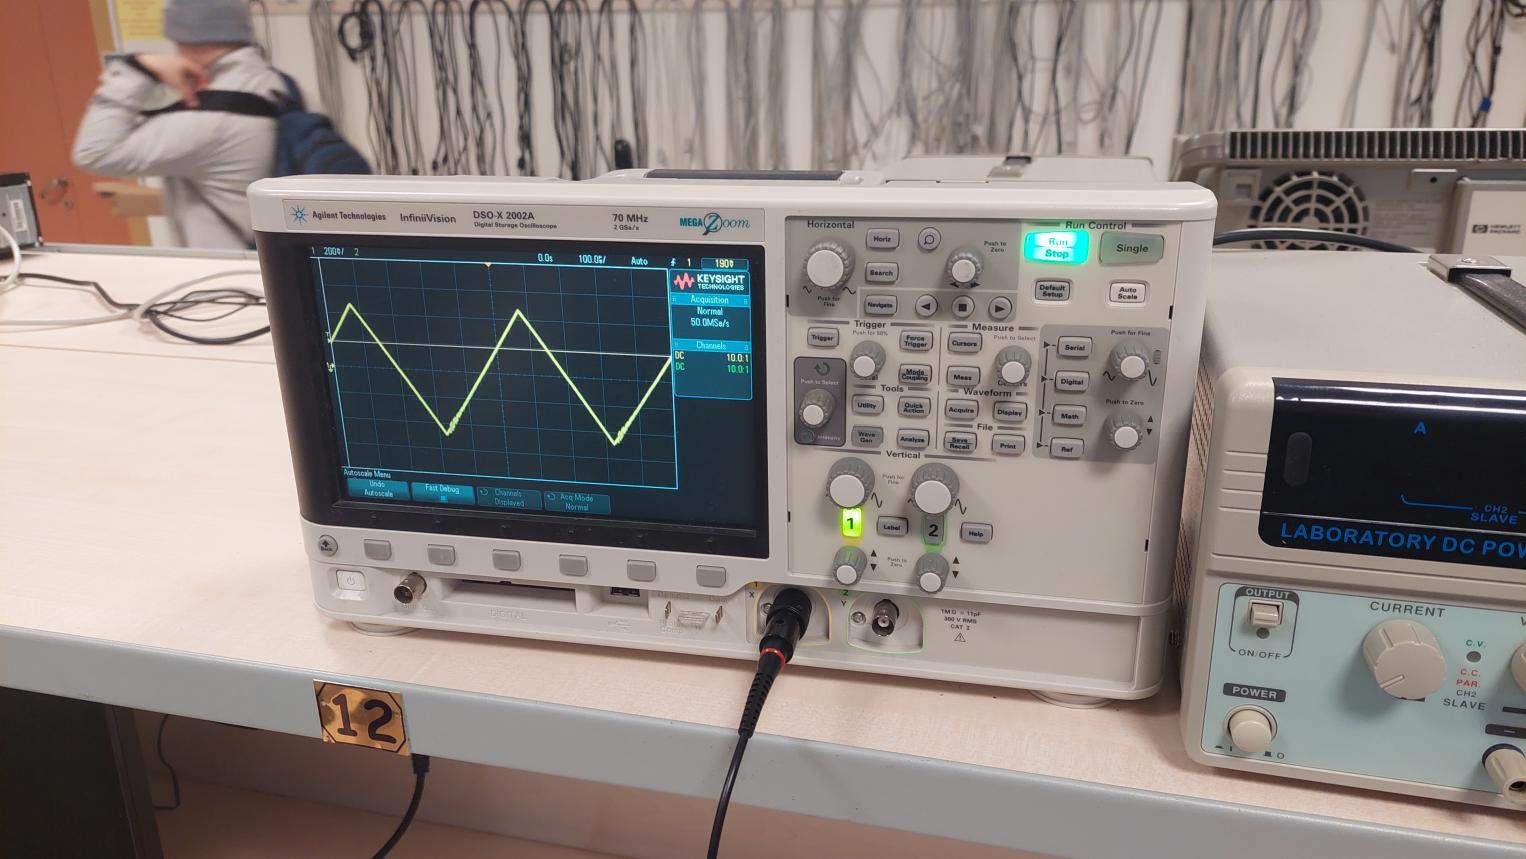
\includegraphics[width=0.48\textwidth]{3.2.jpg}}
	\caption{}
	\label{fig:trig-volt}
\end{figure}

\section{Acquisition Mode, ADC-DAC}

There are many analog signals which need to be probed, but the oscilloscope, like many other computational device, is digital.
This is why a special component named ADC (analog to digital converter) has to be used to make the digital oscilloscope understand the analog signal.

\begin{wrapfigure}{r}{0.5\textwidth}
	\centering
	\subfloat[Normal (Sample)]{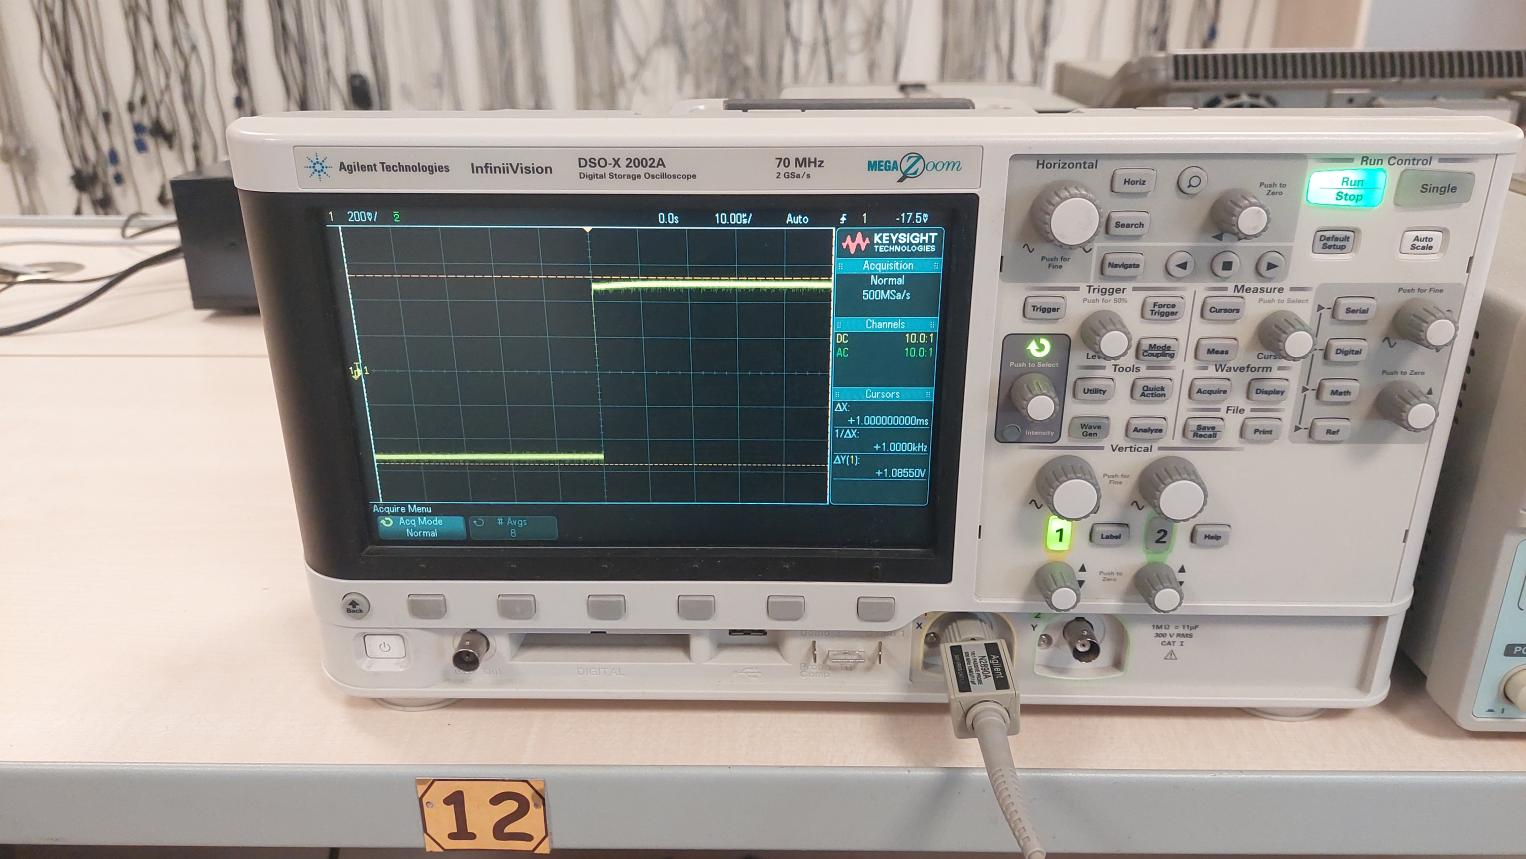
\includegraphics[width=0.4\textwidth]{4.1.jpg}}
	\hfill
	\subfloat[Peak Detect]    {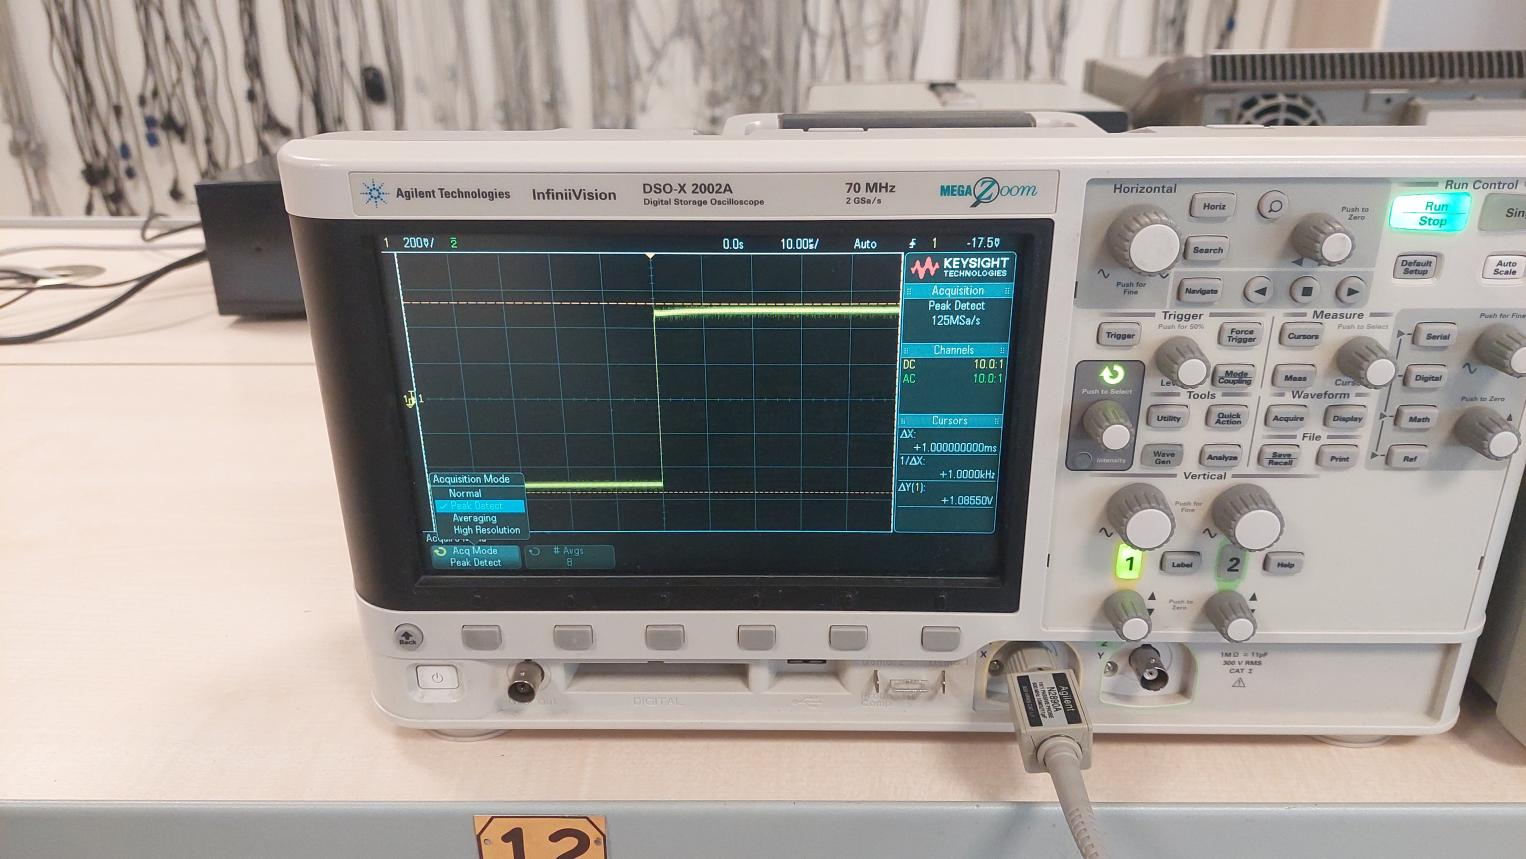
\includegraphics[width=0.4\textwidth]{4.2.jpg}}
	\hfill
	\subfloat[Averaging]      {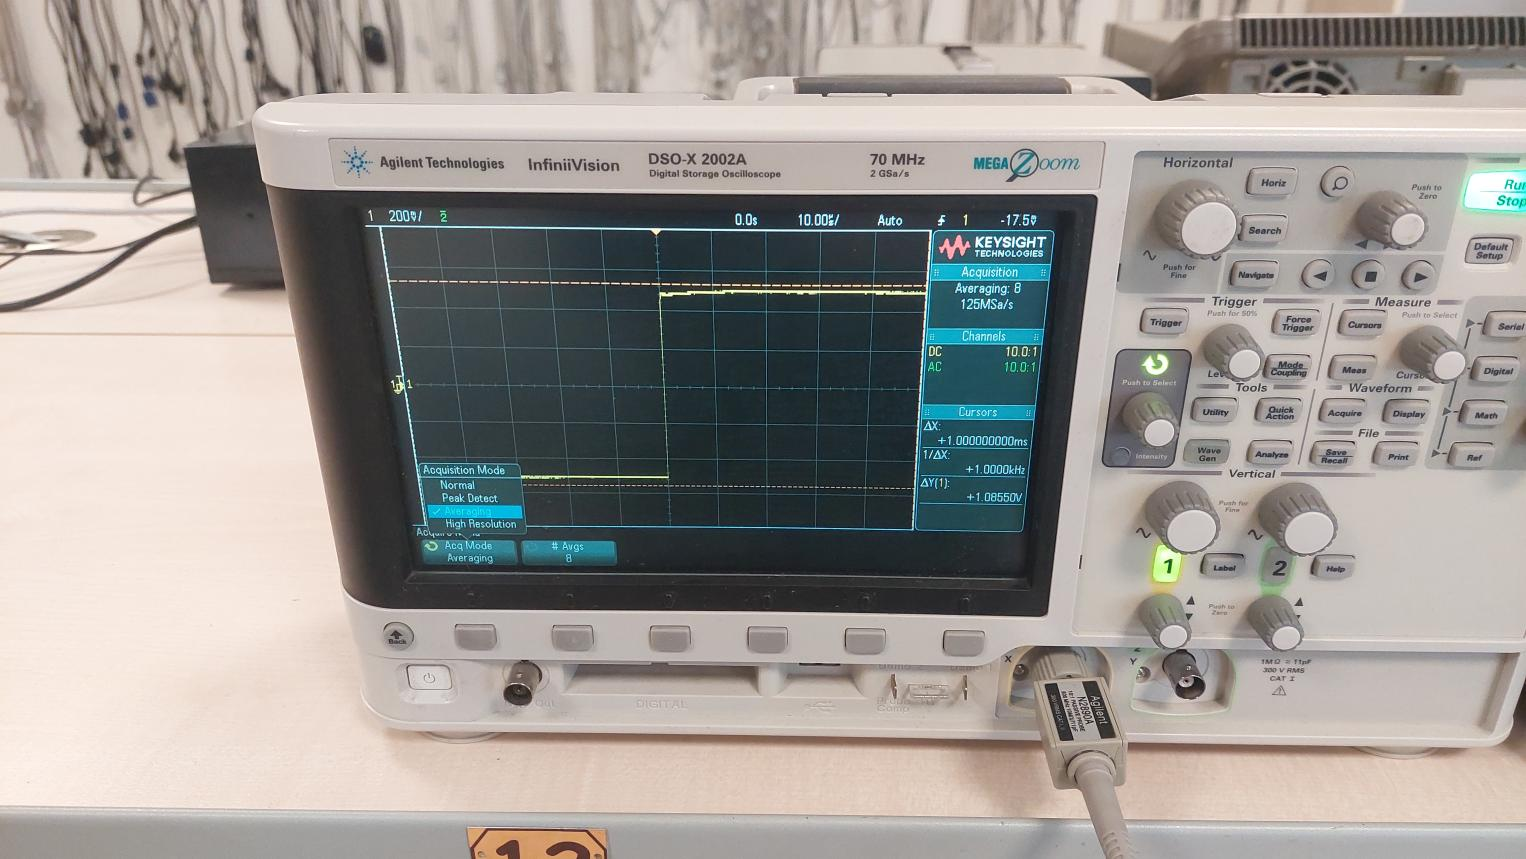
\includegraphics[width=0.4\textwidth]{4.3.jpg}}
	\caption{}
	\label{fig:acq-mode}
\end{wrapfigure}

An ADC, as the name suggests, converts analog signals into digital data, which can then be processed by digital systems (such as the oscilloscope).
The ADC quantizes the analog signal by dividing it into discrete time frames and voltage intervals, then encodes and transmits them to digital processors.
By doing this, some precision is lost, meaning the measurements have maximum frequency and minimum voltage limits, however most oscilloscopes are precise enough for most applications.
The opposite of ADC, DAC (digital to analog converter) converts digital signals into analog waveforms, which the signal generator uses to output various waveforms.

The acquisition modes on the oscilloscope change how the ADC works, changing the processing, and the final image on the screen.
The experiment is done with the signal generator set to 5kHz 1Vpp square wave.
The oscilloscope was initially using the normal (sample) mode, which had noisy peaks and the more vertical parts where the voltage changes rapidly were not clear.
Peak detect mode made the vertical parts more visible,
and the averaging mode completely removed the noise from the high and low parts, as all seen in figure \ref{fig:acq-mode}.

\section{Coupling Mode}

We tell the oscilloscope whether we want to measure a DC or AC signal by setting the coupling mode,
which is for removing a DC offset if trying to measure an AC signal.
When probing a 1kHz 2Vpp sine wave with 1V DC offset (1V added to the original wave) using DC mode, the offset was visible, as it made the plot move up.
However, when AC coupling is used for probing the same signal, the vertical offset was gone and the 0V line was passing through the middle of the sine wave, as seen on figure \ref{fig:acdc-coup}b.
Using the AC coupling mode allow to see the AC aspect of a signal more clearly.

\begin{figure}[!h]
	\centering
	\subfloat[DC Coupling]{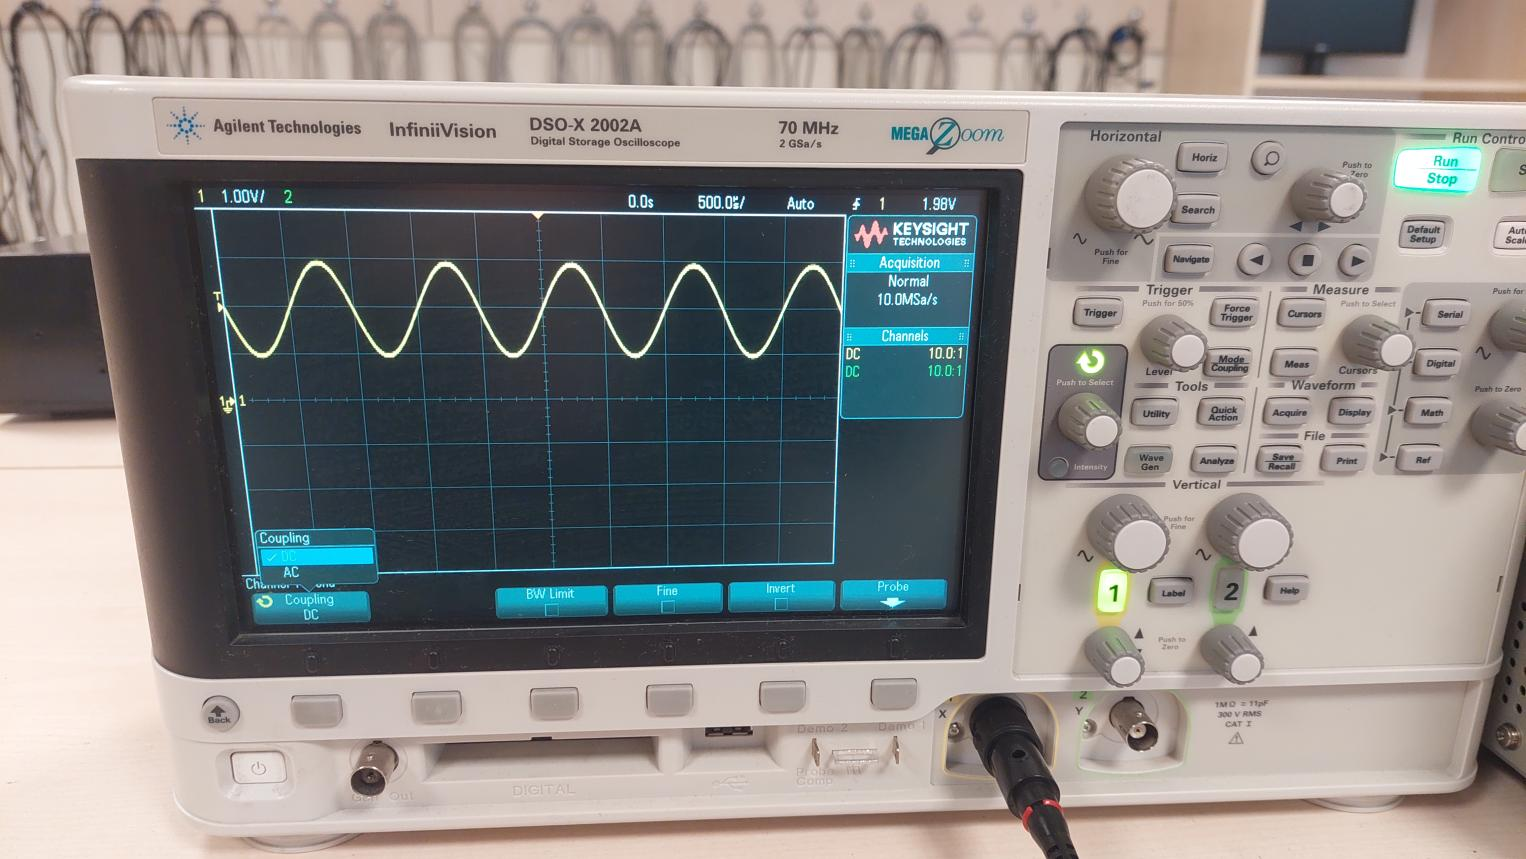
\includegraphics[width=0.48\textwidth]{5.1.jpg}}
	\hfill
	\subfloat[AC Coupling]{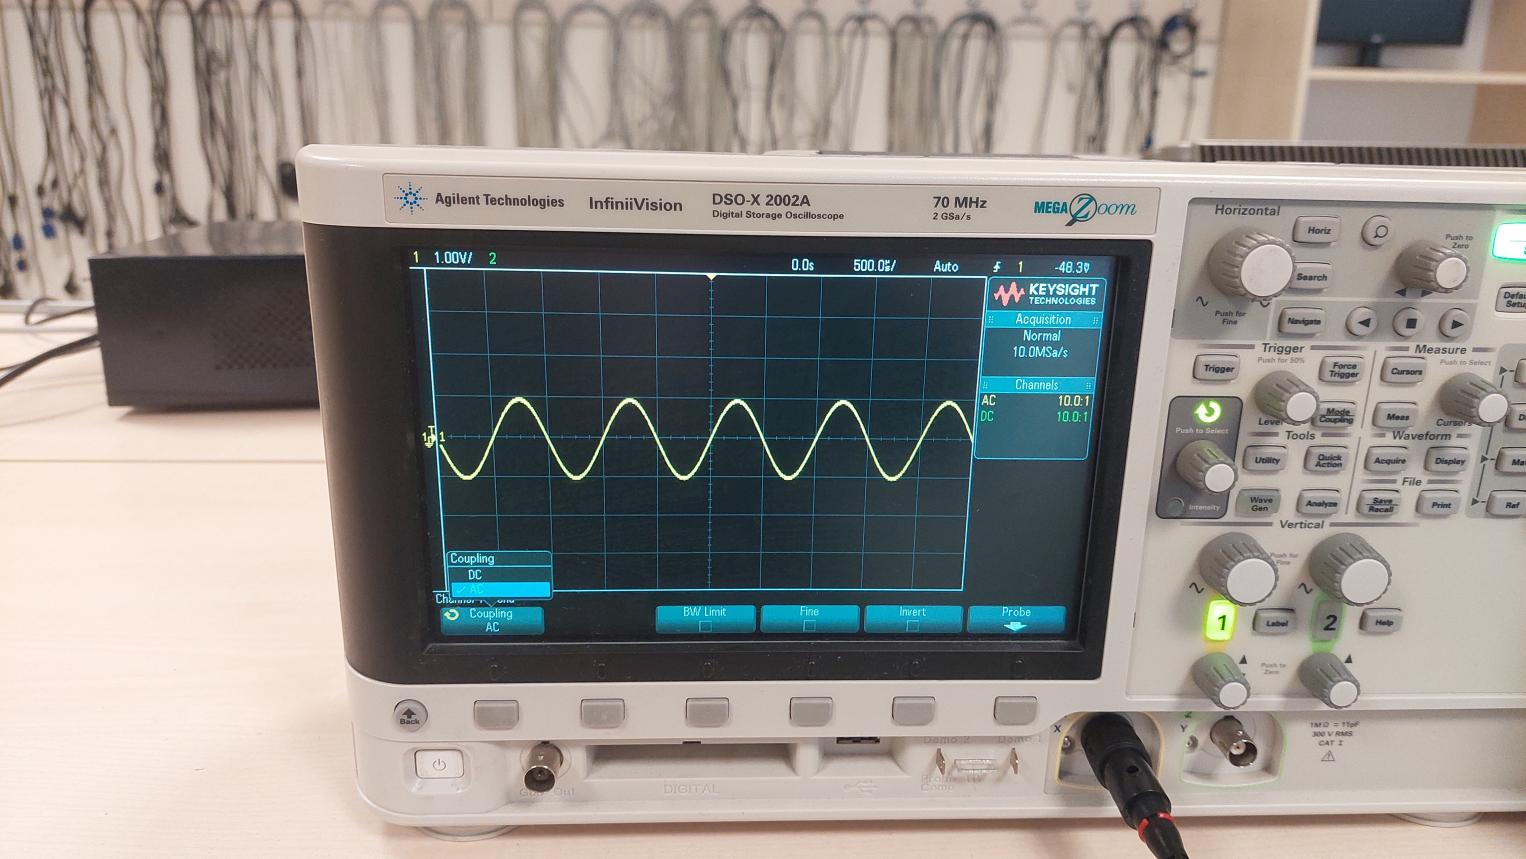
\includegraphics[width=0.48\textwidth]{5.2.jpg}}
	\caption{}
	\label{fig:acdc-coup}
\end{figure}

\section{6}

\begin{wrapfigure}{r}{0.5\textwidth}
	\centering
	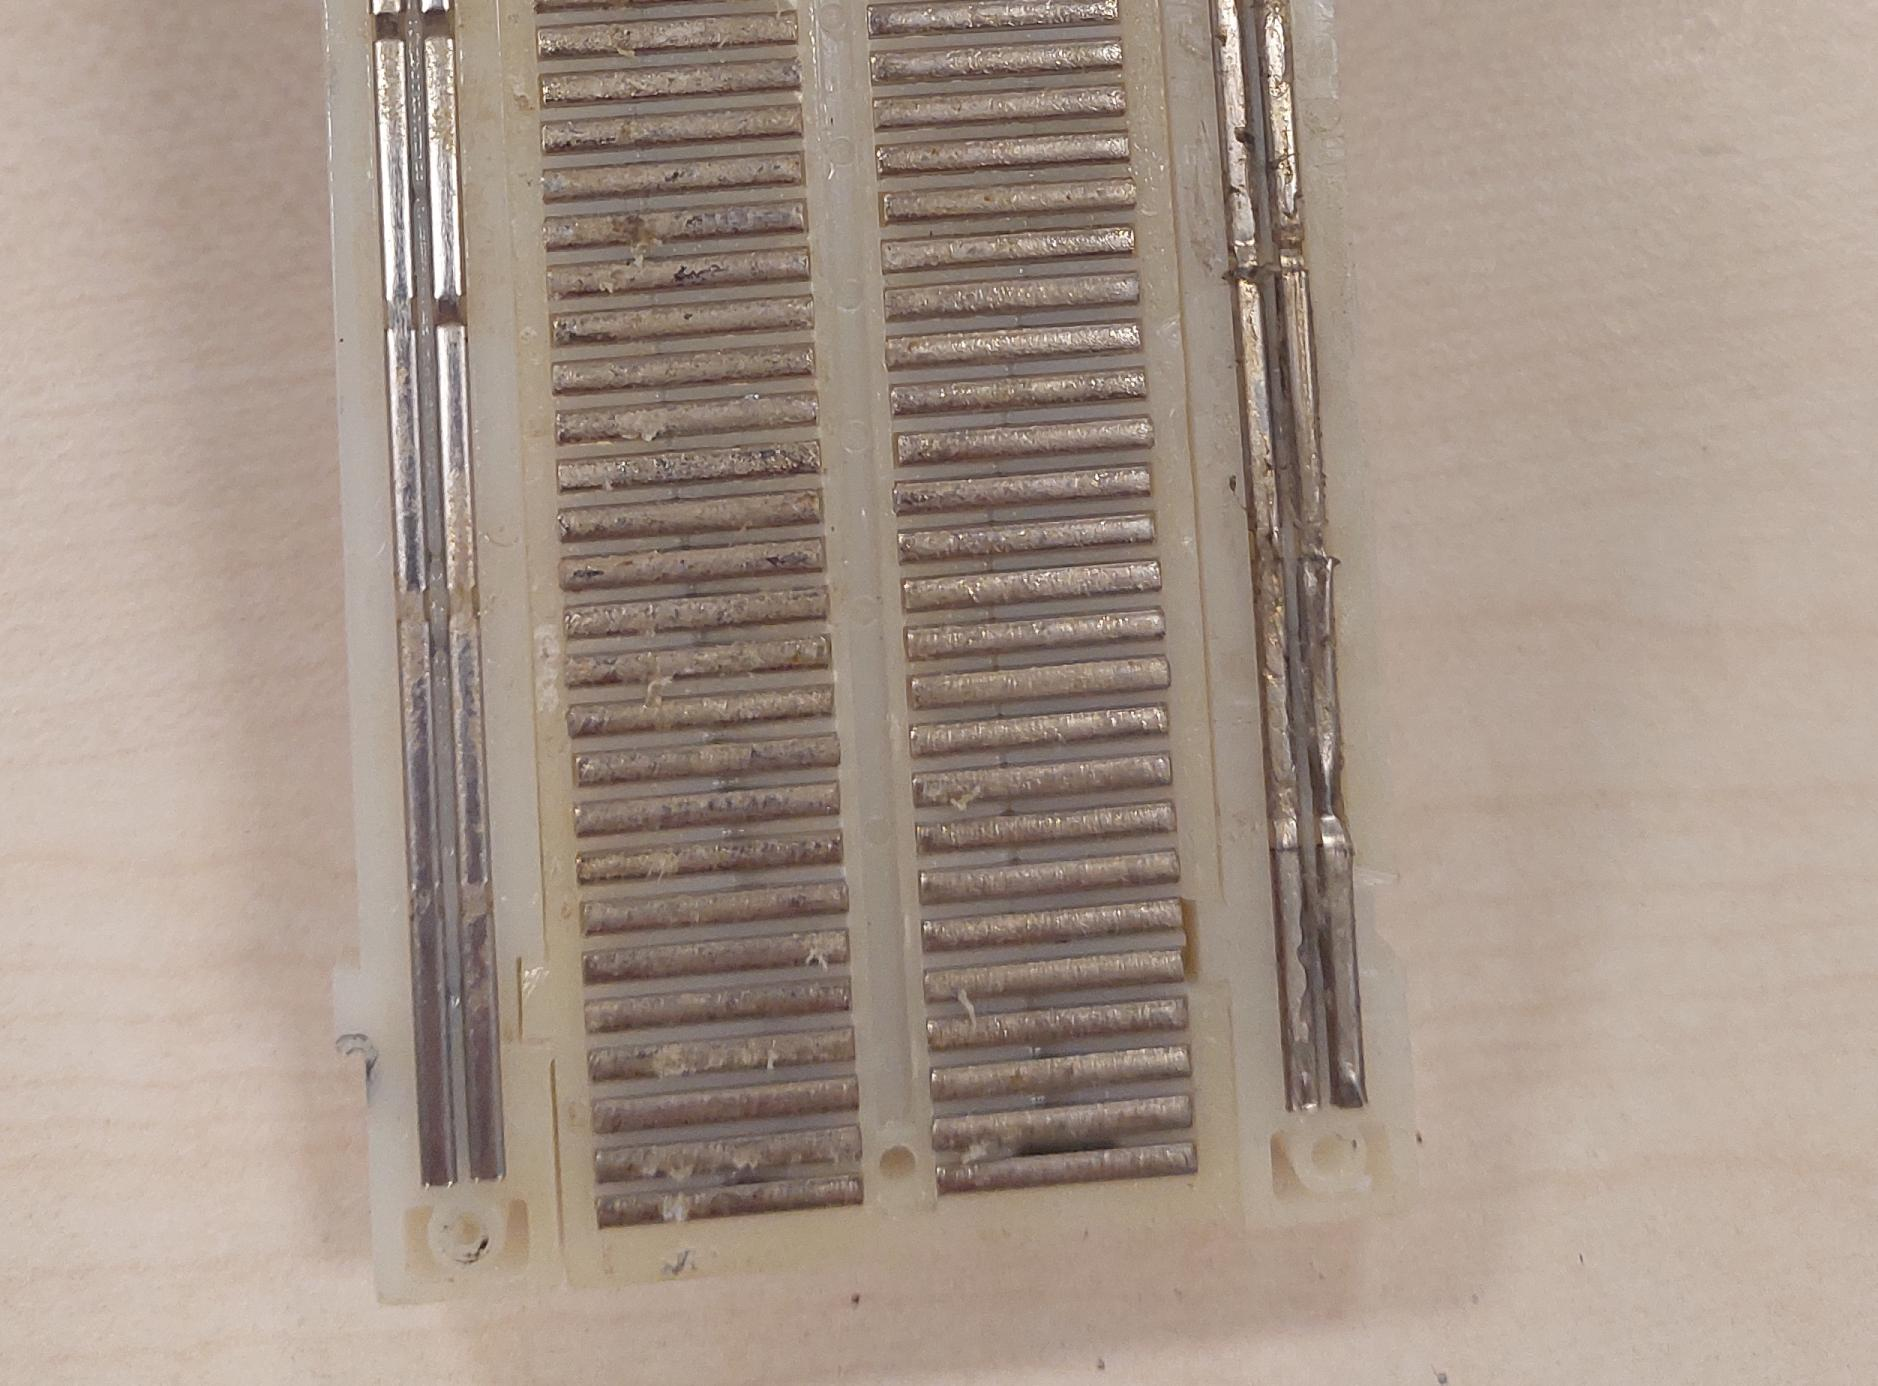
\includegraphics[width=0.4\textwidth]{6.0.jpg}
	\caption{Breadboard, from behind}
	\label{fig:breadboard}
\end{wrapfigure}

A breadboard is an electronics prototyping tool, on which components can be placed and connected, without soldering.
On a typical breadboard, behind the component-leg holes, there are metal pieces which electrically connect each row, where components are placed, hence connecting them.

\begin{figure}[!h]
	\centering
	\subfloat[Circuit Schematic]{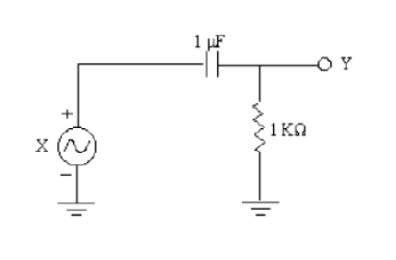
\includegraphics[width=0.4\textwidth]{6.1.jpg}}
	\hfill
	\subfloat[Assembled Circuit]{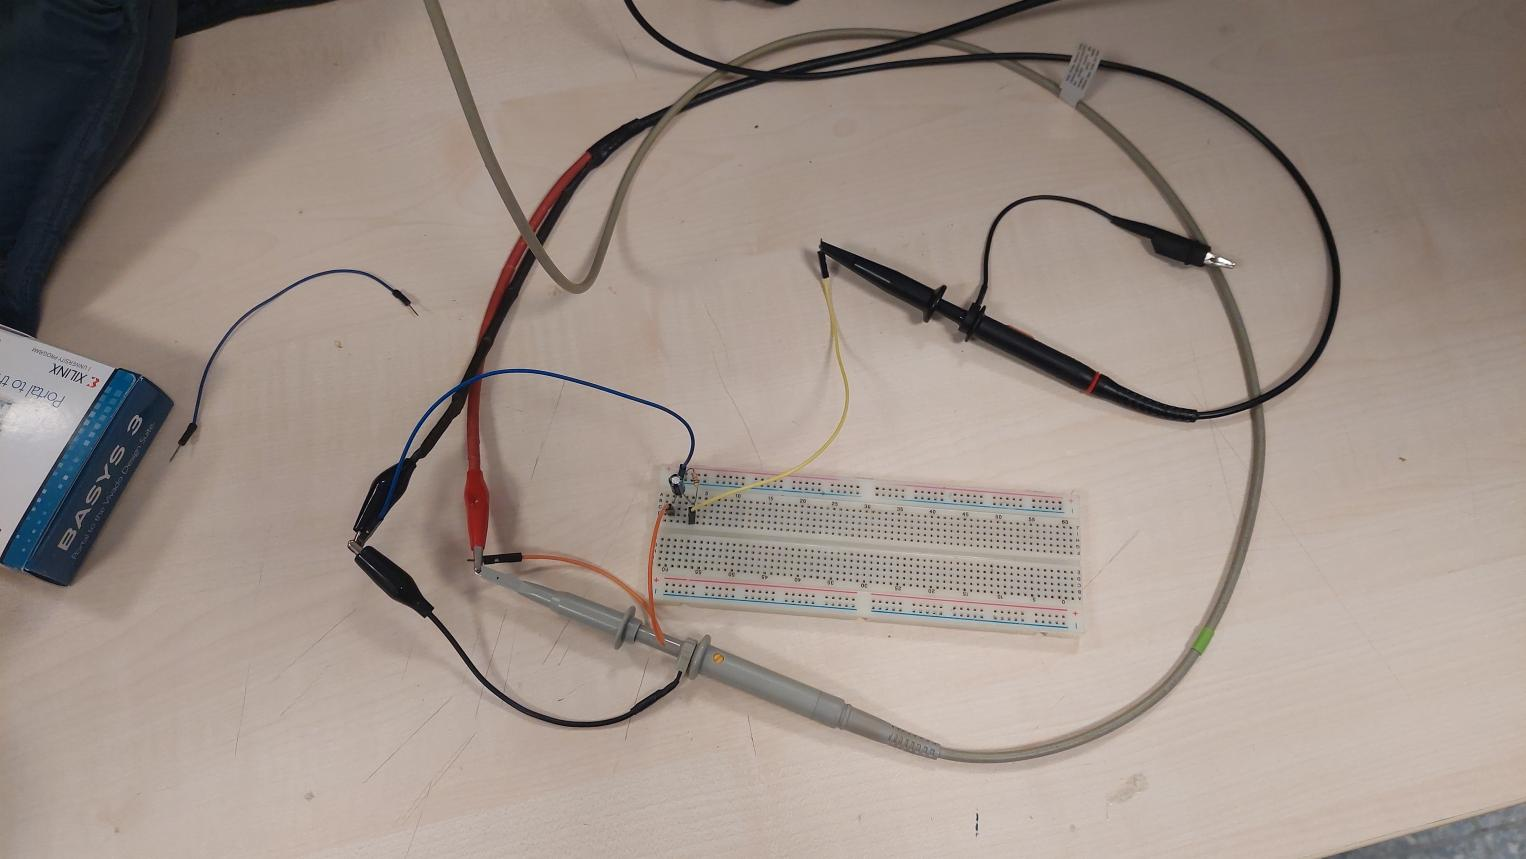
\includegraphics[width=0.48\textwidth]{6.2.jpg}}
	\caption{}
	\label{fig:circuit}
\end{figure}

The circuit on figure \ref{fig:circuit} is assembled on the breadboard and connected to the oscilloscope and the signal generator.


When the signal generator is set to 1Khz 2Vpp sine wave, there signal Y can be seen to lag behind signal X 33$\mu$s which is a 12\degree phase shift.
However, when the frequency is increased to 100kHz, there is no visible phase shift and the two signals perfectly overlap, as seen on figure \ref{fig:phase}.

\begin{figure}[!h]
	\centering
	\subfloat[1kHz]{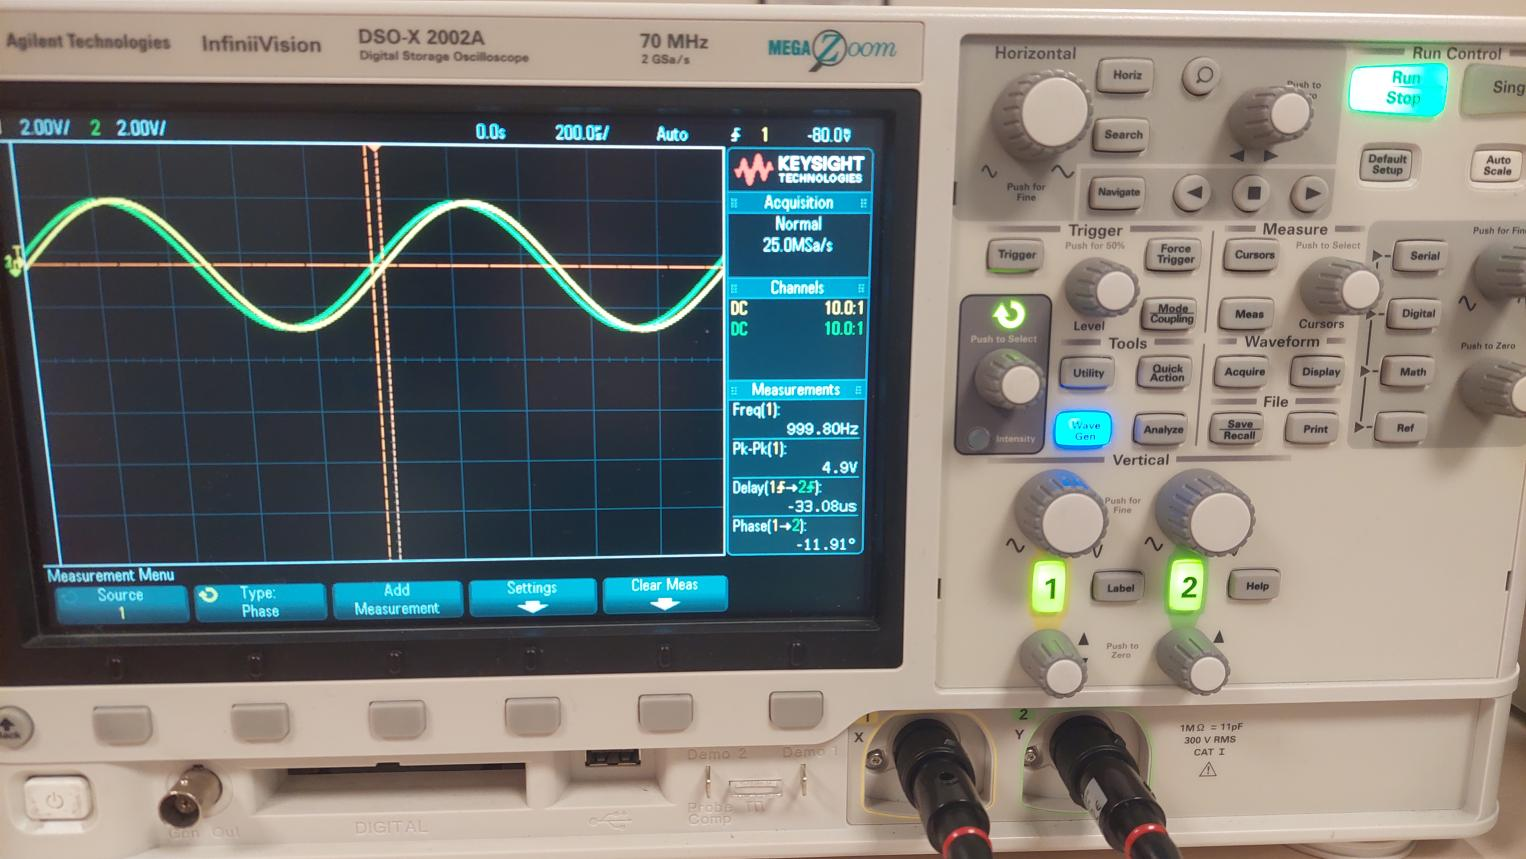
\includegraphics[width=0.4\textwidth]{6.3.jpg}}
	\hfill
	\subfloat[100kHz]{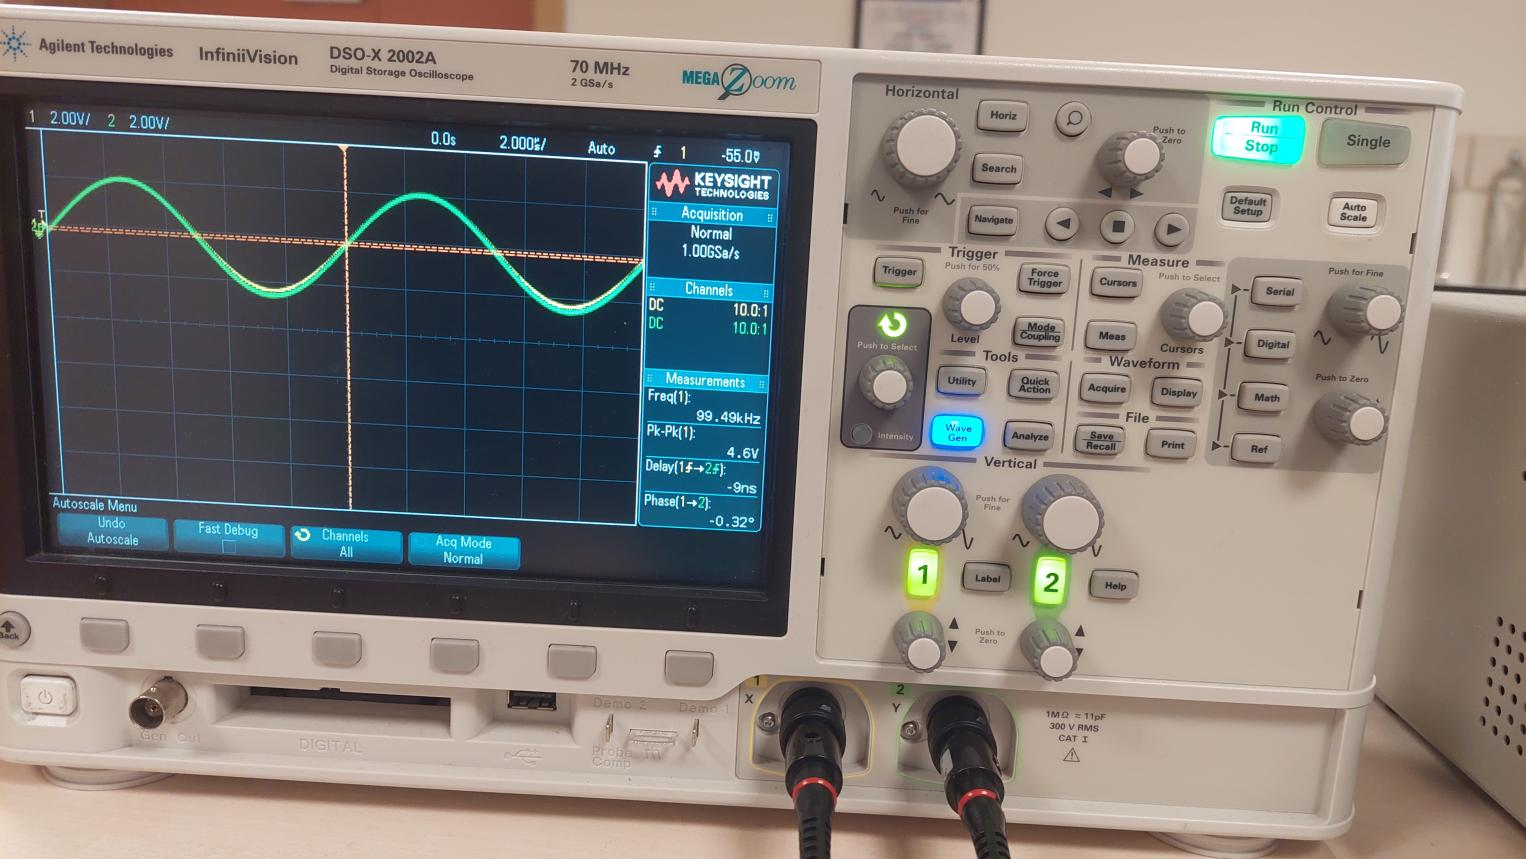
\includegraphics[width=0.48\textwidth]{6.4.jpg}}
	\caption{}
	\label{fig:phase}
\end{figure}

The phase difference may be due to the capacitor in the circuit adding extra delay to the signals.

\end{document}
